\normalfont\normalsize
\chapter{Evaluation}

Our goal was to deliver a solution that could be deployed in an application as fast as possible, so
instead of running software simulations, we decided to implement and test the algorithm on the new
node Sparrow R. The algorithm is implemented in C, and compiled with gcc-arm-none-eabi-4.8.3-2014q1 on Arduino 1.6.4.

We selected 2 super-capacitors of 1F and 5V maximum rating, one using Electrolytic Double
Layer (EDLC) technology and other using Aerogel technology. We fully charged the capacitor and then
let the algorithm decide how fast the data should be transmitted in order to reach the time
deadline.

The only input needed is the current voltage of the capacitor, read using a voltage divider that is
controlled by an n-mos transistor in order to reduce the power dissipated by the divider. The node
will run a task that simulates sensors readings and other processing through a delay of 100 ms. The
network is configure as single-hop, and the data sent through RF has the length of 45 bytes.

\begin{figure}[ht] \centering
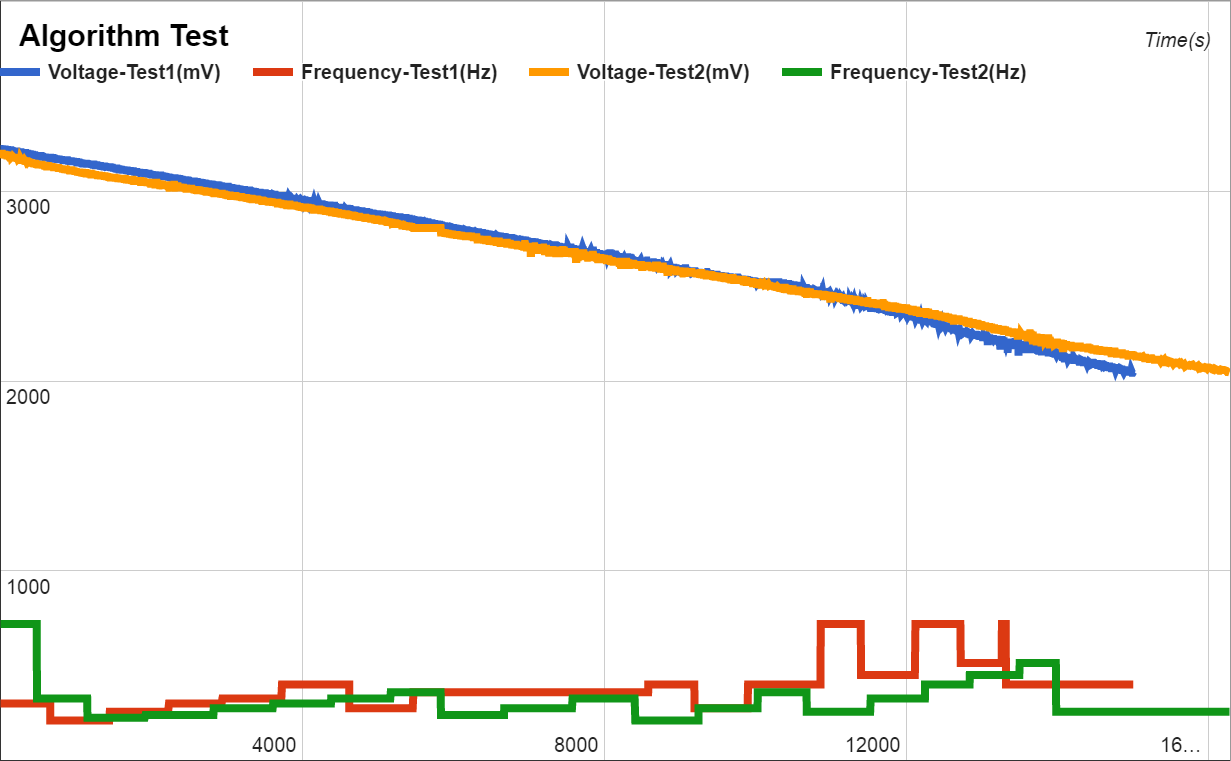
\includegraphics[width=0.85\textwidth]{img/algtest.png}
\caption{Two runs of the algorithm with EDLC capacitor and 4 hours deadline}
\end{figure}

When beginning with a deadline of 4 hours, in the first run, the node manages to execute 1593 task and be
functional for a total time of 4 hours and 18 minutes. The second run, with a new deadline of 4
hours and 11 minutes, the node ran 1631 tasks for a total time of 4 hours and 35 minutes.

With a longer, more realistic deadline of 8 hours, the node managed to transmit 785 times for a
duration of 8 hours and 14 minutes.

$$E = E_i - E_f = 3.24J$$
$$P_{4h} = \frac{E}{T_{4h}} = \frac{3.24J}{258 * 60s} = 209uW $$
$$P_{8h} = \frac{E}{T_{8h}} = \frac{3.24J}{494 * 60s} = 109uW $$

The algorithm is working, the average power for the 8 hours is twice as small as the one for the 4
hours. Unfortunately, the total number of send data is twice as small, which indicates that the
combined power used by the node when sleeping and the leakage of the capacitor is starting to
influence the total number of sent data.

We ran into problems when a longer deadline of 12 hours was tested, mainly because the self
discharge of the capacitor combined with the idle current
consumption of the node is high enough to waste more than 75\% of the energy. This had a significant
impact on the total number of executed tasks. The first run of the test send data 143 times and
lasted for 13 hours and 10 minutes. The second run started with a more realistic speed of 10 task
per hours instead of 600, but the total number of sent data dropped to 18 with a total duration of
13 hours and 15 minutes.

The 12 hours test meant that 1F capacitor is barely enough for 12 hours with our demo test and that
a bigger capacitor might be needed. Because we had two types of 1F capacitor, we were curios to
see if there is a difference between them. What we found was a bit of surprise, especially the
lowest voltage at which the node stopped working. The Aerogel capacitor had a lower voltage of 1950mV
compared to the ELDC of 2050mV. However, the EDLC capacitor managed to transmit more data than
the Aerogel, even when the algorithm was tweaked to take into consideration the lower working
voltage of the Aerogel capacitor. The EDLC managed to send data 1642 times, while the Aerogel one manage only
1254 times.

\begin{figure}[ht] \centering
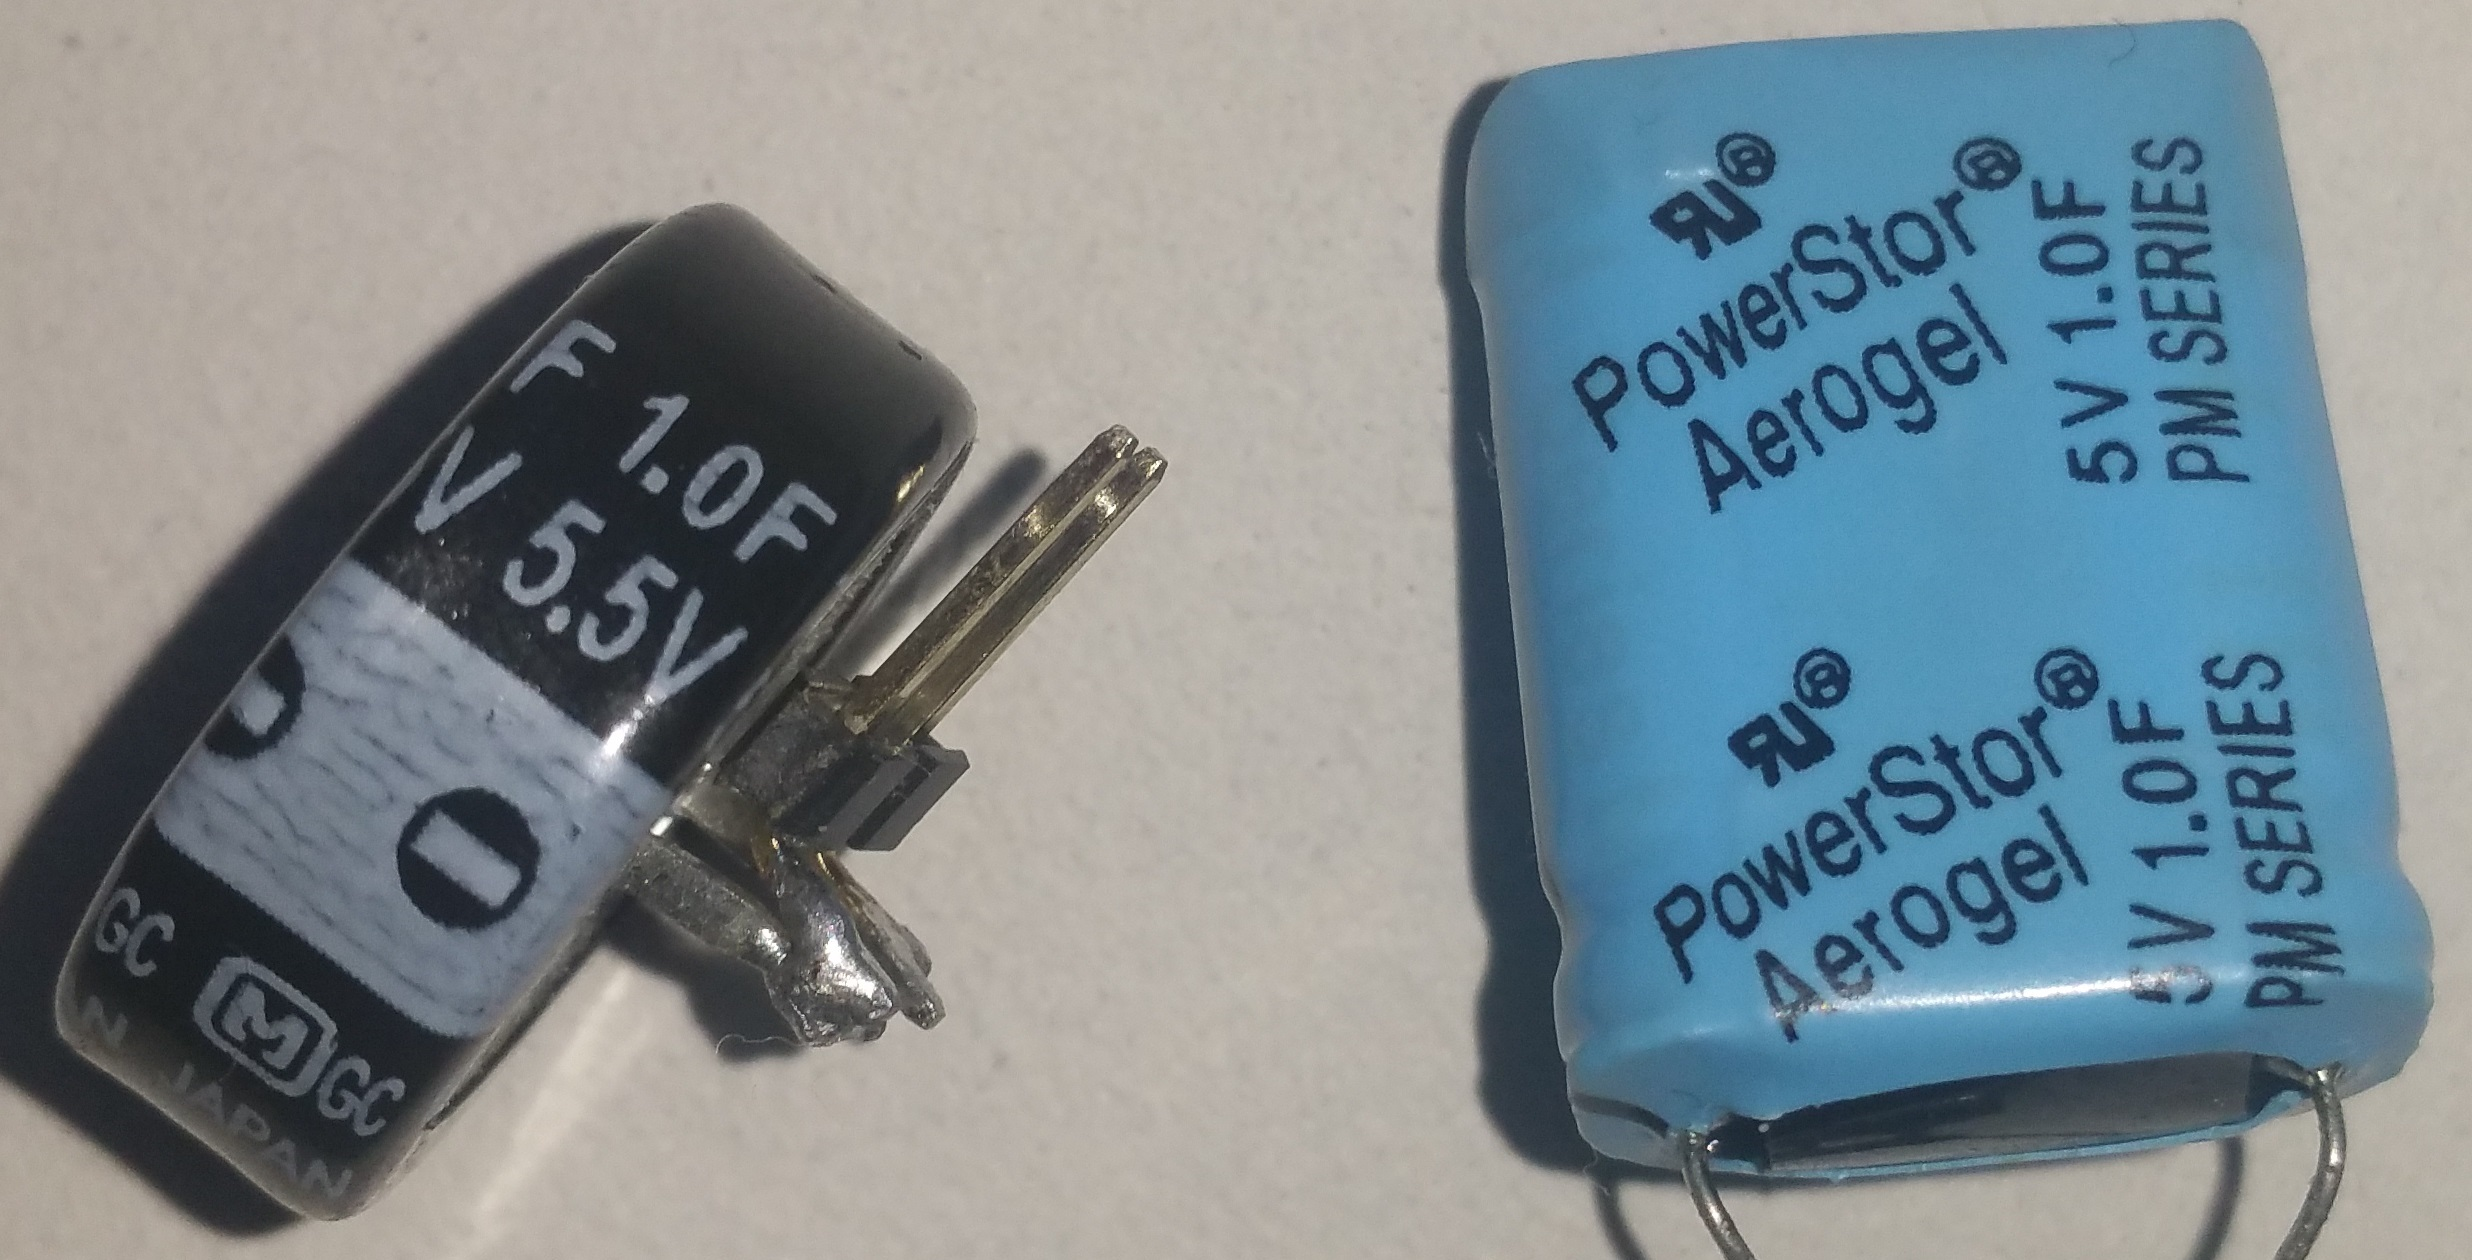
\includegraphics[width=0.85\textwidth]{img/capacitors.jpg}
\caption{1F different capacitors, Left EDLC - Right Aerogel}
\end{figure}

\begin{figure}[ht] \centering
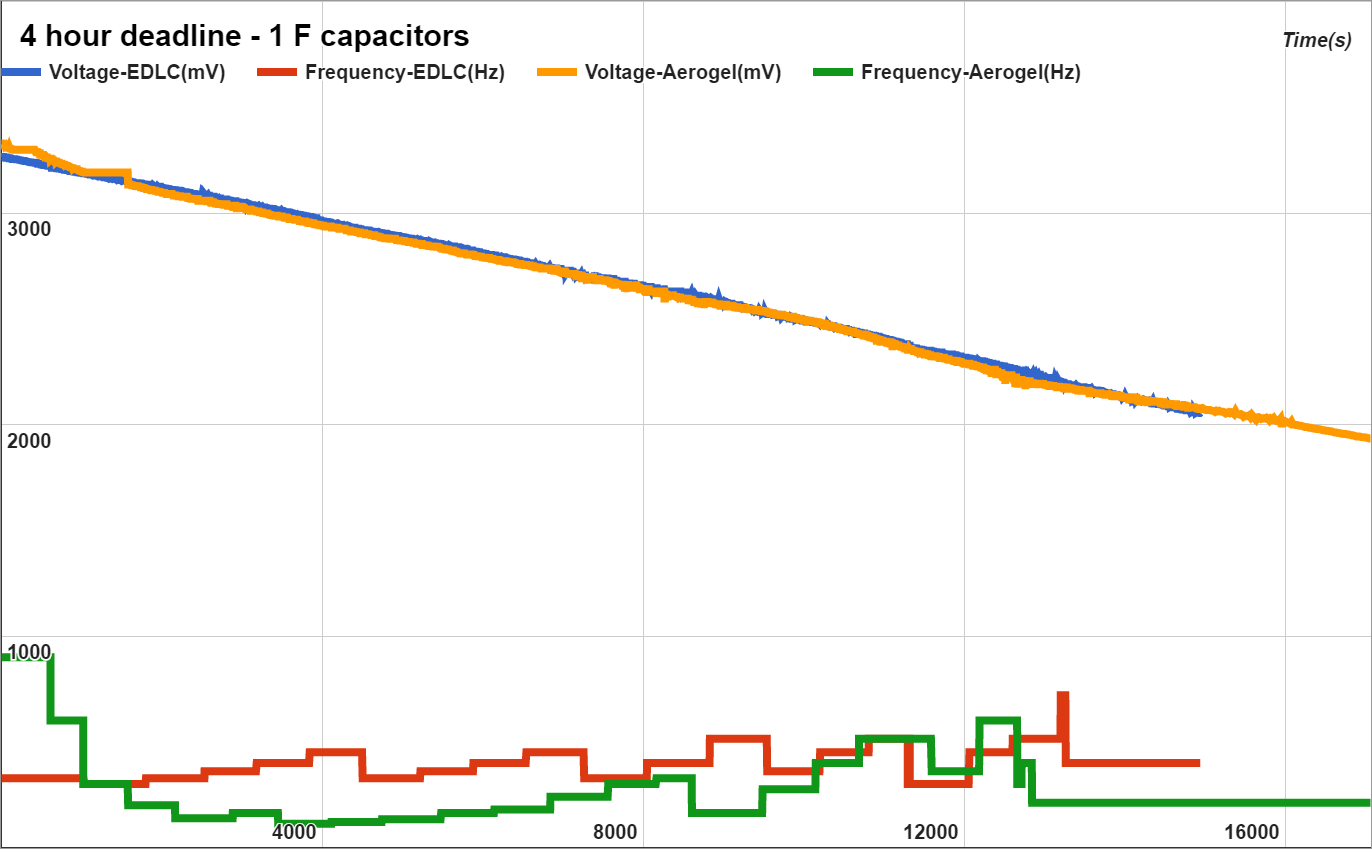
\includegraphics[width=0.85\textwidth]{img/captest1.png}
\caption{1F different capacitors test, Aerogel vs EDLC}
\end{figure}


